
\ChapterWithSubtitle{Modeling Climate Change}{now we can swim any day in november}
%\chapter{Heating by Radiation}

%%%%%%%%%%%%%%%%%%%%%%%%%%%%%%%%%%%%%%%%%%%%%
\section*{Equipment List}

\begin{multicols}{2}   % change 2 -> 3 for three columns
\begin{equipment}
\item Computer (lab-provided or your own)
\end{equipment}
\end{multicols}


%%%%%%%%%%%%%%%%%%%%%%%%%%%%%%%%%%%%%%%%%%%%%
\section{Introduction}

Today we will explore an online climate simulation tool, called {\bf En-ROADS}\footnote{\url{https://en-roads.climateinteractive.org/scenario.html}}, created by MIT Sloane School of Management and the ``environmental think tank''  \href{https://www.influencewatch.org/non-profit/climate-interactive/}{\em Climate Interactive}. You should have watched their 10~min ``Overview and Introduction'' video\footnote{Located in 2025 at \url{https://www.youtube.com/watch?v=4O-5fsVZaII}} already, but you could refresh yourself now with the 2~min ``Overview'' video at {\em Help/Video Tools/EN-ROADS Overview}\footnote{We will explore this tool and try to become familiar with it, but if you would like to train yourself more deeply you could take their online course \url{https://learn.climateinteractive.org/course/mastering-en-roads}.}.  Your reading this week from Dessler (Chapter 8: {\em Predictions of Future Climate Change}) will also help you to understand the definitions and methods of quantities used in this modeling tool.

To get started, take 10--15 min to play with the tool, exploring the options for adjusting the parameters (both using the adjustable bars, and opening the setting to manully control the numbers), visualizing different output graphs, and determining outcomes that differ from the ``baseline'' presented.  Talk with the lab partners at your table about what you are finding and share methods on how to access all of the tools/options.  While/after doing so, write a brief paragraph that answers most of the following questions.
	%
	\begin{itemize}
	\item What is the basic idea of this tool?  What are the inputs and what are the outputs?
	\item Where are the connections to our prior study of climate change, e.g., ``climate sensitivity'', the connection between increasing $\text{CO}_2$ in the atmosphere and temperature rise?
	\item What else is incorporated in the tool, other than these climate physics principles?  (I would say it accounts for the science, but also societal and economic factors. How?)
	\item Explain the plot shown in the 10~min En-ROADS introduction video (at 4:54, reproduced below), in which En-ROADS is compared to NGFS.  What does the graph show? What is NGFS and why are they comparing to it? What are the three different scenarios plotted? (You might need to look some things up online!)
	\end{itemize}

\vfill

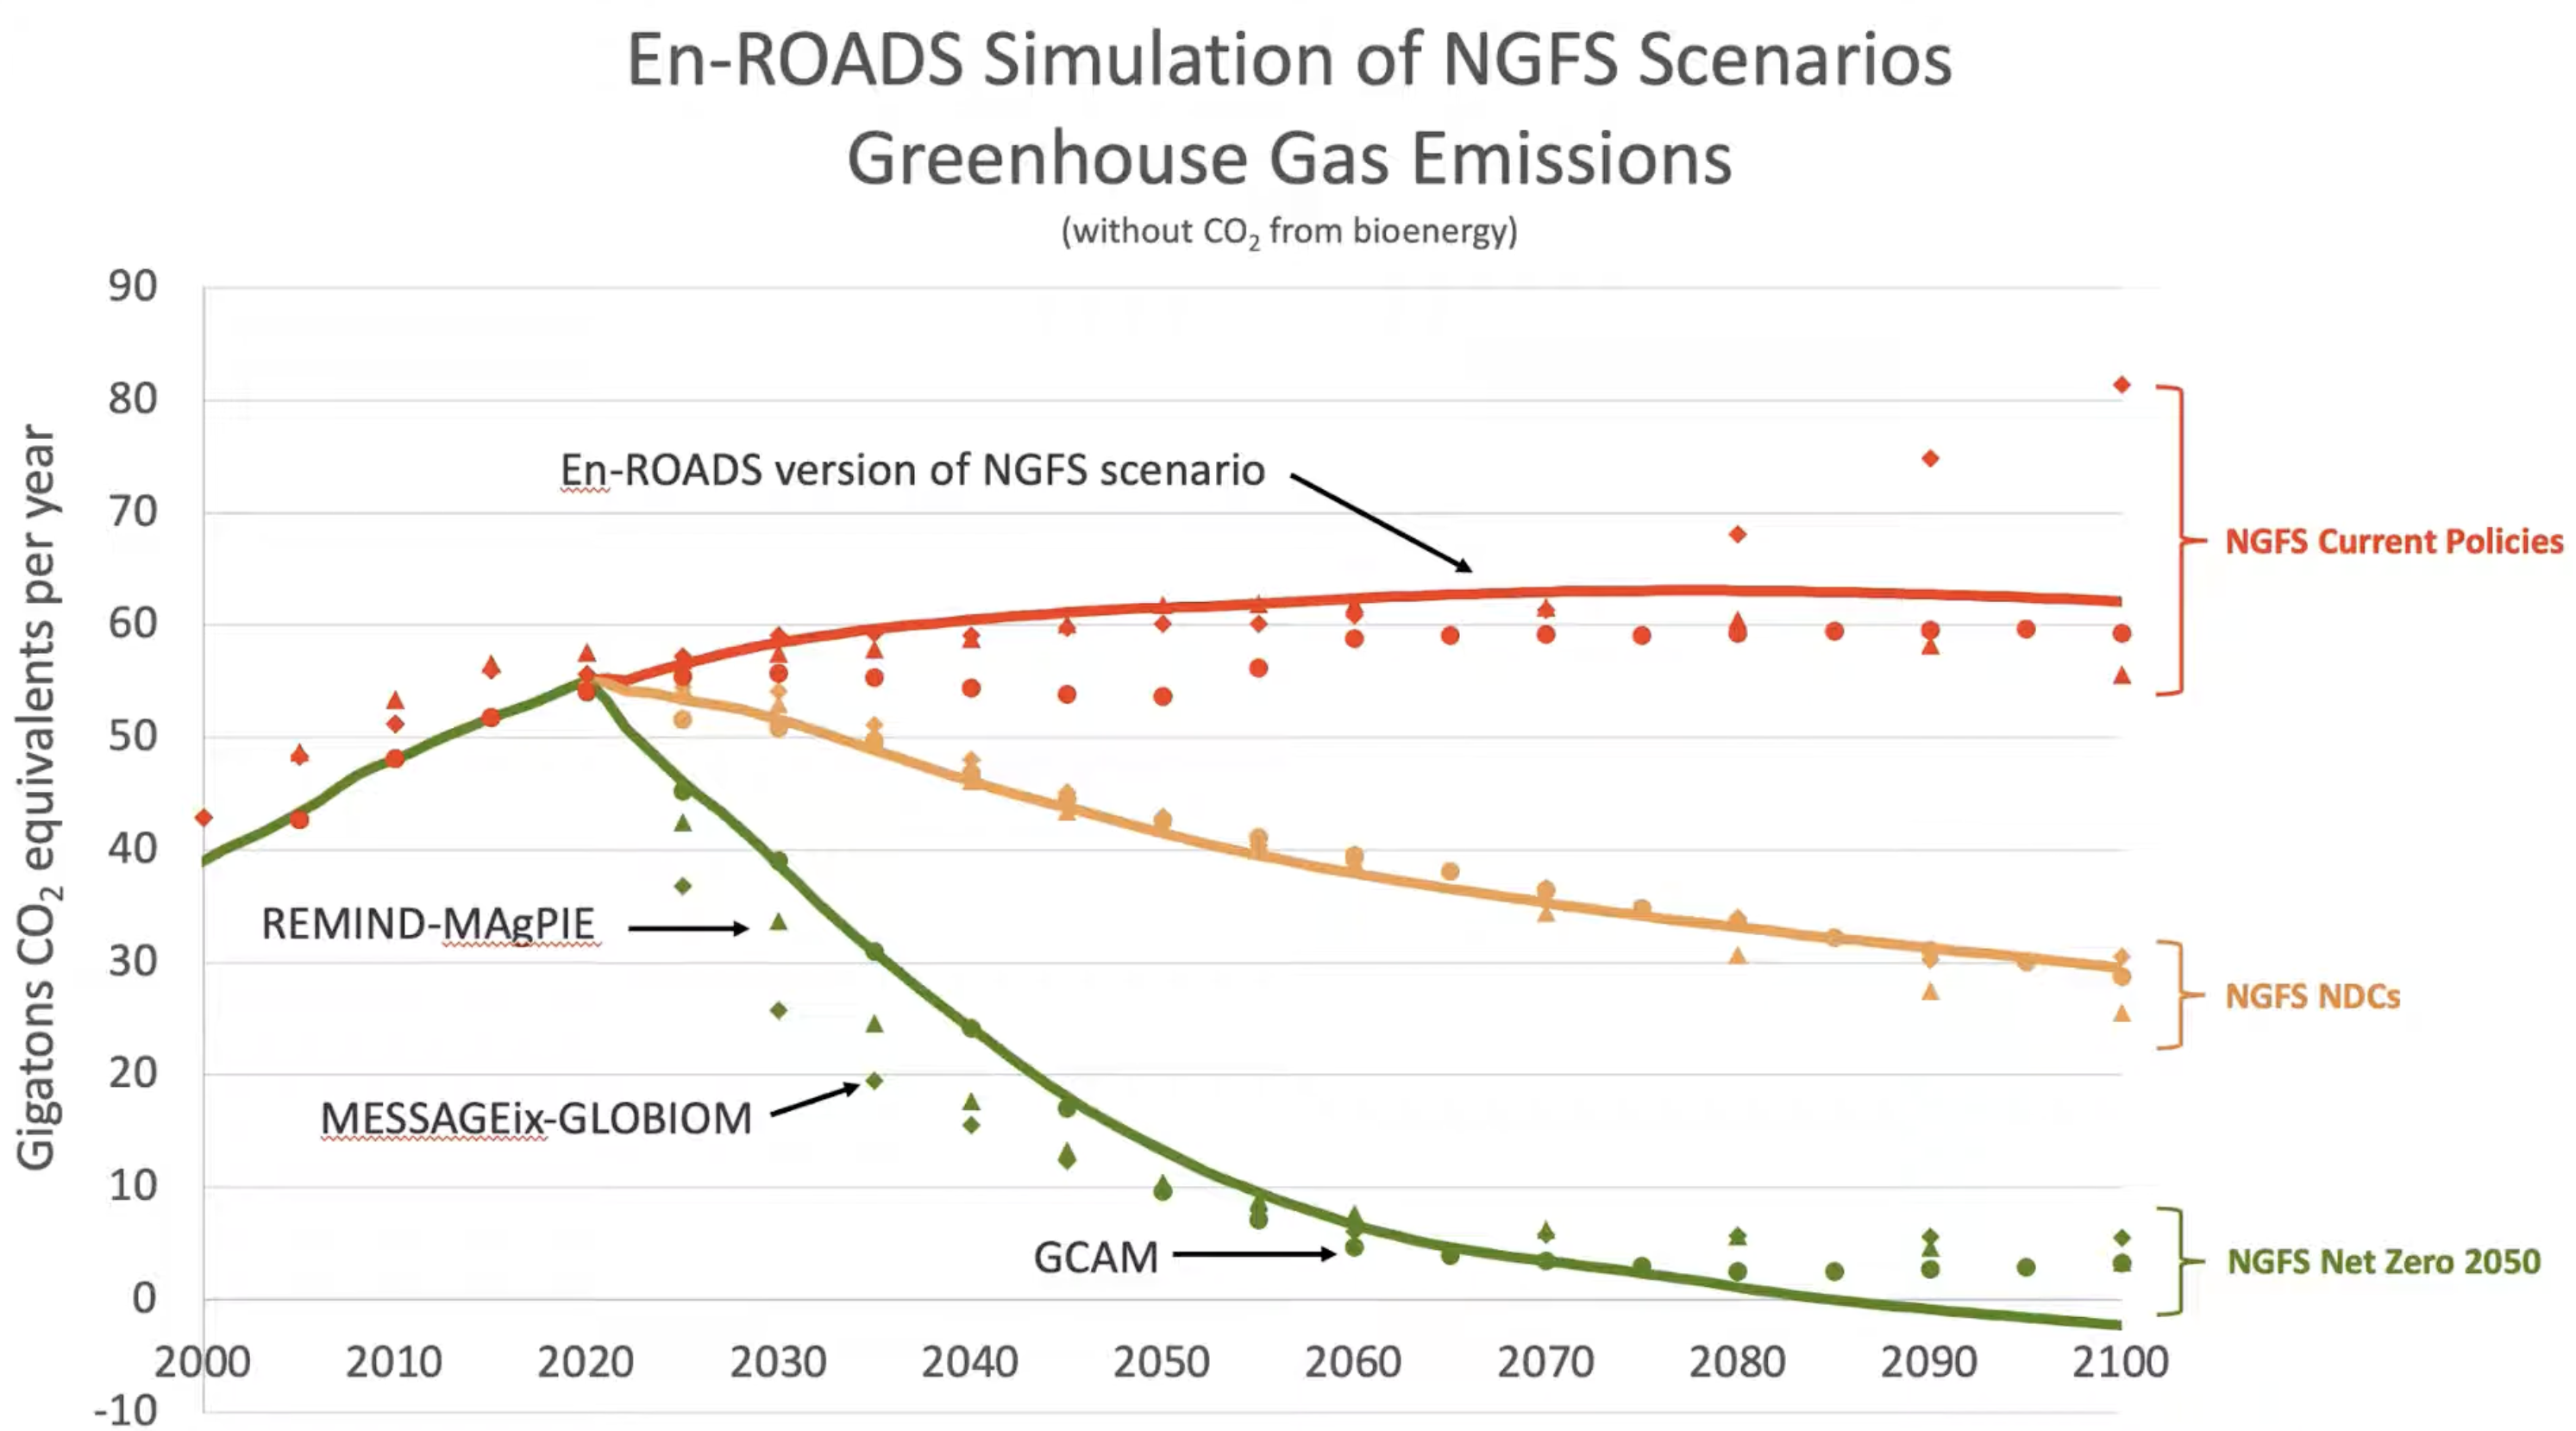
\includegraphics[width=\textwidth]{images/10_enroads-comparison-to-ngfs.png}

\newpage
%%%%%%%%%%%%%%%%%%%%%%%%%%%%%%%%%%%%%%%%%%%%%
\subsection{Identifying the climate science elements of the simulation}

In its default setup, the En-ROADS simulation shows a panel of two graphs and a temperature value (click the Home and reset icons to return to default).  Describe these three displays and explain their meanings.

\answerspace[7cm]

\noindent The primary outcome shown, {\em Greenhouse Gas Net Emissions}, is not a quantity we have explored before.  It would be useful to put it into context with other more familiar quanties (like atmospheric $\text{CO}_2$ concentrations and average temperature).  Using your own piece of graph paper, make a graph with {\em four} vertical axes (two on each side) showing these data sets\footnote{You should be able to find each of these datasets at \url{ourworldindata.com}, but access each individual plot {\bf by Googling} for, e.g., ``ourworldindata cumulative co2 emissions'' (the ourworldindata internal search engine is bad, so be sure to use google to access these plots).  Once at the data graph, remove all country data (``Clear'') and select only the ``World'' dataset; limit the time range using the slider.} --- Annual $\text{CO}_2$ emissions, Cumulative $\text{CO}_2$ emissions, Annual temperature anomaly, and atmospheric $\text{CO}_2$ (ppm) ---  and a horizontal axis showing time from 1975 to 2025.  \\[-6pt]

\noindent Examining your graphs, explain how our familiar quanties (atmospheric carbon dioxide and global temperature) relate to the emissions annual quantity plotted in En-ROADS.

\answerspace[5cm]

%%%%%%%%%%%%%%%%%%%%%
\newpage
\noindent Considering your own graphs, do you see any evidence for the statement\footnote{See, e.g., Figure 1b in Jeevanjee et al (AREPS 2025) and the related discussion.} that ``temperature is proportional to cumulative emissions''?

\answerspace[5cm]

\noindent What is the implication of this proporionality for the increase in temperature prior to a halt of $\text{CO}_2$ emissions, and the behavior of the temperature after the halt of $\text{CO}_2$ emissions?  Discuss this refererencing the figures shown below from Dessler Chapter 8.


\vfill

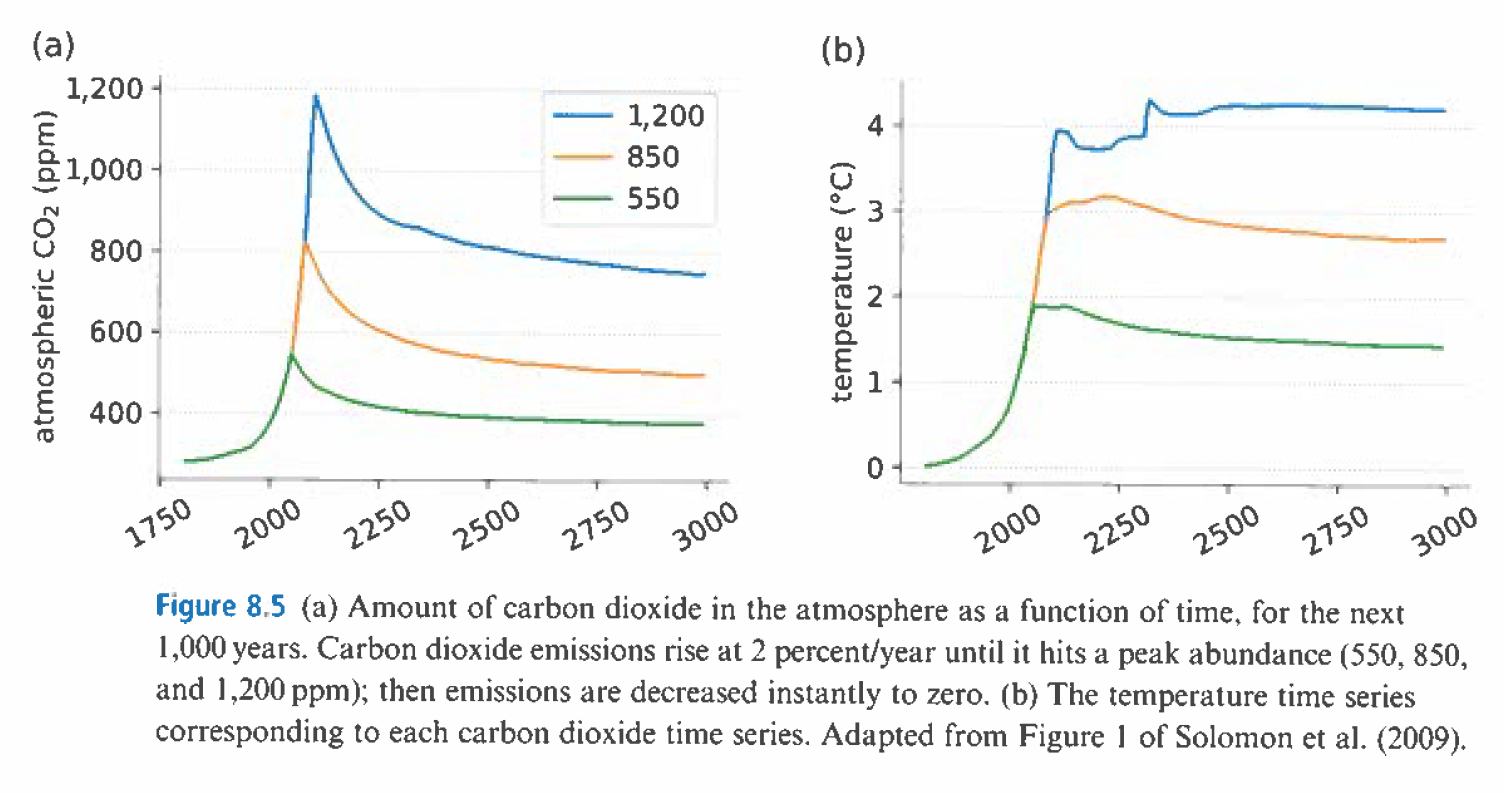
\includegraphics[width=\textwidth]{images/10_dessler_fig8-5.png}

%%%%%%%%%%%%%%%%%%%%%
\newpage

\noindent Returning to the simulation, let's examine the climate science inputs to the model and their effects on temperature.  There are three such parameters in the model, listed under {\em Simulation / Assumptions / Earth System / Climate System Sensitivities}.  List these quantities (one should be familiar to you, the other two we have not yet discussed) and define them based on information given at the model page and/or your own brief online research.  


\answerspace[7cm]

\noindent  Now use the {\em Assumptions} page to adjust these quantities and investigate their impact on the temperature graph.  Which has the most influence?  If we assume a $\pm 0.5\degree$C uncertainty in the ``Climate Sensitivity'', how much uncertainty does that lead to in the temperatures at 2050 and 2100?







 